\chapter{Aplicaciones}

\noindent Se han podido aprovechar los fractales áreas como: Matemáticas, Física, Química, Comunicaciones, Informática, Geología, Economía, Música, Biología, etc…\\

\section{Fractales en la naturaleza}

\noindent Los fractales se pueden encontrar en la naturaleza, por ejemplo, en la forma de las hojas, las ramas de los árboles, las venas de las hojas, las costas, las montañas, los copos de nieve, los relámpagos, los cristales, etc.\\

\noindent Si conseguimos identificar una estructura fractal en un fenómeno natural, podemos estudiar de forma matemática su comportamiento a futuro, permitiendo explicar procesos complejos con fórmulas relativamente simples (como ya vimos en la generación con L-systems)\\

\section{Aplicaciones en la biología}

\noindent Los fractales, además de ser usados en el estudio del crecimiento de las plantas, son usados en:

\begin{itemize}
    \item El estudio de problemas pulmonares, ya que los pulmones presentan una estructura fractal para repartir el aire de forma homogénea.\cite{BBVA-2020}
    
    \begin{figure}[H]
        \centering
        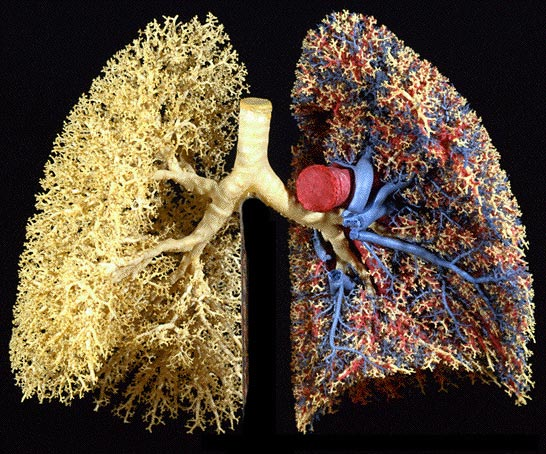
\includegraphics[width=0.5\textwidth]{figures/lungs-fractal.jpg}
        \caption{Estructura fractal de los pulmones.} \cite{BBVA-2020}
        \label{fig:lungs}
    \end{figure}

    \item La evolución de especies depreadoras en entornos controlados pueden representar patrones fractales. \cite{fractales-img}
    
    \item El estudio del ADN y los enlaces entre nucleótidos. \cite{ADN}.
    
    \begin{figure}[H]
        \centering
        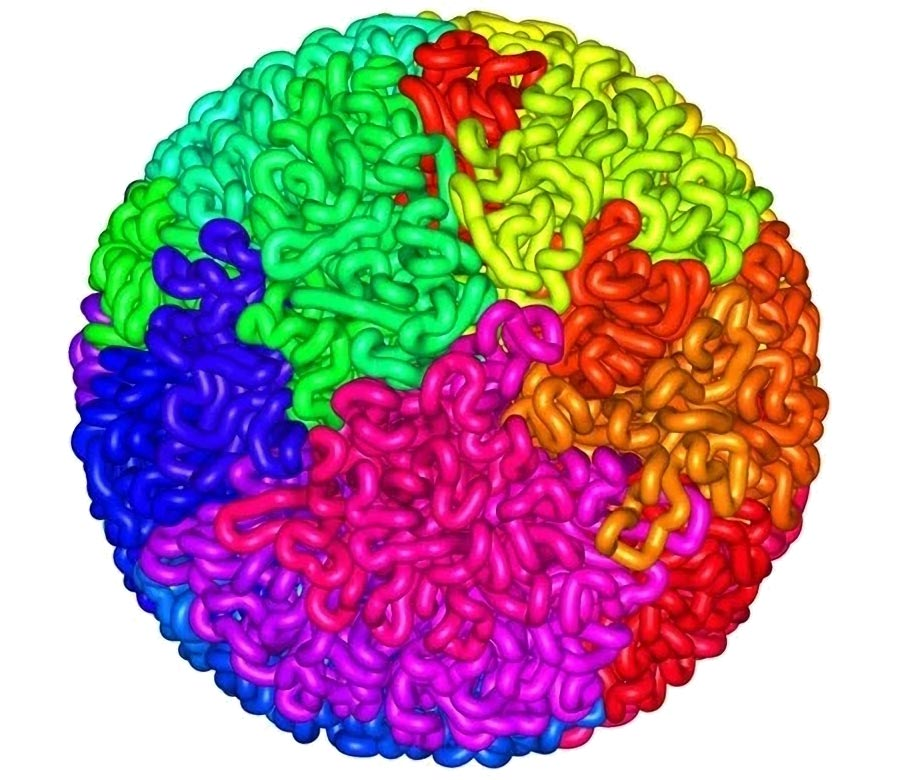
\includegraphics[width=0.5\textwidth]{figures/fractal-genome.jpg}
        \caption{Imagen de como el ADN se compacta en una estructura fractal}
        \label{fig:fractal-genome}
    \end{figure}
\end{itemize}

\section{Aplicaciones en comunicaciones}

\noindent En comunicaciones e informática se experimenta con la compresión fractal de archivos para que ocupen menos espacio.\cite{compresion-fractal} \\

\begin{figure}[H]
    \centering
    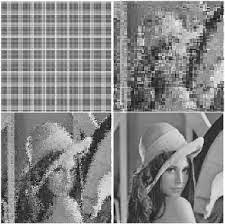
\includegraphics[width=0.5\textwidth]{figures/fractal-compression.jpeg}
    \caption{Ejemplo de compresión fractal}
    \label{fig:fractal-compression}
\end{figure}

\noindent También se ha experimentado con las redes de ordenadores con estructura fractal para comprobar si generan mejor rendimiento. \cite{fractales-img}

\section{Aplicaciones en la geología}

\noindent En la geología, se usan para estudiar las irregularidades de la costa y relieves del terrenos, además de la distribución de las islas y continentes.\cite{BBVA-2020}\\

\begin{figure}[H]
    \centering
    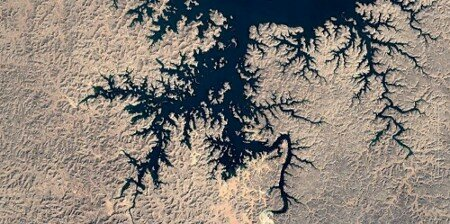
\includegraphics[width=0.5\textwidth]{figures/Lake-Nasser.jpeg}
    \caption{Lago Nasser, Egipto}
    \label{fig:lake-nasser}
\end{figure}

\noindent Los terremotos tienen una relación fractal entre la intensidad del terremoto y la frecuencia del suceso. \cite{geologia}\\

\section{Otras aplicaciones}

\noindent Los fractales también se usan en:

\begin{itemize}
    \item La ecología, para cuantificar los niveles de CO2 que procesan los bosques. \cite{BBVA-2020}
    \item La astrofísica, para estudiar la formación de estrellas.\cite{BBVA-2020}
    \item La economía, para estudiar el comportamiento de la bolsa.\cite{BBVA-2020}
    
    \begin{figure}[H]
        \centering
        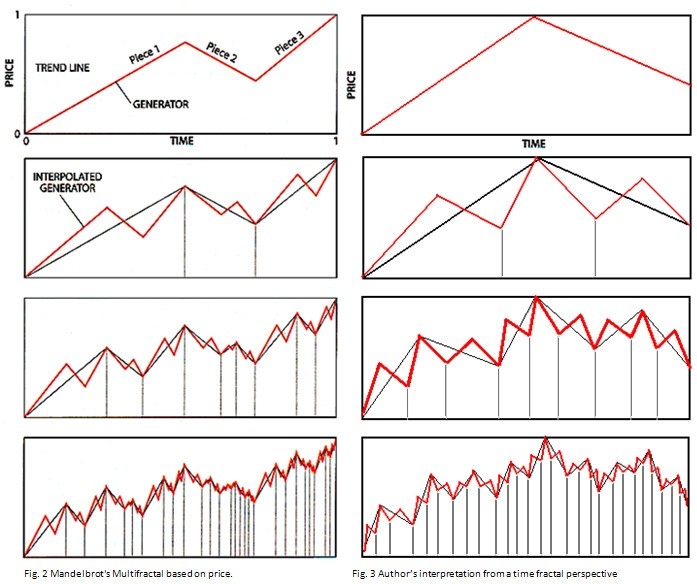
\includegraphics[width=0.5\textwidth]{figures/fractal-economy.jpg}
        \caption{Fractal financiero}
        \label{fig:fractal-economy}
    \end{figure}

    \item Gráficos por ordenador, para generar texturas y paisajes.
    
    \begin{figure}[H]
        \centering
        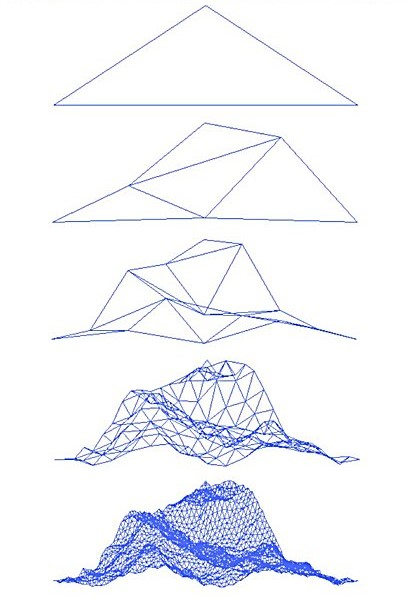
\includegraphics[width=0.5\textwidth]{figures/fractal-mountain.jpg}
        \caption{Fractal que genera una montaña}
        \label{fig:fractal-mountain}
    \end{figure}

\end{itemize}
